% Supplementary Material — ACM Multimedia Asia 2026
% Paper: PanoDive360: A Novel Equirectangular Projection Dataset and
%        Enhanced Attention Mechanism for Underwater 360-Degree
%        Multiclass Semantic Segmentation
%
% Compile (Overleaf or local):
%   pdflatex PanoDive360_supplementary.tex
%
% For CMT double-blind review, comment the \author line.
\documentclass[11pt,a4paper]{article}

\usepackage[margin=1in]{geometry}
\usepackage{times}
\usepackage{graphicx}
\usepackage{booktabs}
\usepackage{tabularx}
\usepackage{amsmath}
\usepackage{hyperref}
\usepackage{caption}
\usepackage{subcaption}
\usepackage{xcolor}
\usepackage{enumitem}

\hypersetup{colorlinks=true,linkcolor=black,citecolor=black,urlcolor=blue}

\title{\textbf{Supplementary Material}\\[0.4em]
\large PanoDive360: A Novel Equirectangular Projection Dataset and Enhanced Attention Mechanism for Underwater 360-Degree Multiclass Semantic Segmentation}
\author{Ghulam Arbi \quad Lu Zhang \quad Yanyong Zhang\\
University of Science and Technology of China}
\date{ACM Multimedia Asia 2026}

\begin{document}
\maketitle

\begin{abstract}
\noindent
This supplement records the reproducibility protocol and the extra
experiments that do not fit in the 6-page ACM main paper: random-seed
robustness (seeds 42, 123, 777), training/validation curves, and ERP
video-inference cost. All numbers match the PanoDive360 chapter graphs.
Code: \url{https://github.com/aiguo112/PanoDive360}.
\end{abstract}

\section{Reproducibility protocol}
\label{sec:protocol}

\subsection{Software and hardware}
All models were implemented in Python~3.8.19 with PyTorch~1.8.0,
CUDA~11.1 and cuDNN~8902.
Training used dual NVIDIA GeForce RTX~3060 GPUs (12~GB each) with
data parallelism.
Latency and FPS in Table~\ref{tab:compute} were measured on an
RTX~5070~Ti: batch size~$=1$, 20 warm-up iterations, 100 timed
iterations, CUDA synchronised, input padded to $1440\times736$.

\subsection{Training hyperparameters}
Table~\ref{tab:hyper} lists the protocol applied identically to
U-Net, U-Net++, PSPNet, DeepLabv3+ and ERP-CBAM.
The paper resolution is $1440\times720$ (2:1 ERP, no crop).
The public \texttt{panodive360/config.py} currently defaults to a
square $1024\times1024$ resize; that setting does \emph{not} reproduce
the paper tables. Override it to $(1440,720)$ before rerunning.

\begin{table}[t]
\centering
\caption{Training hyperparameters on PanoDive360.}
\label{tab:hyper}
\begin{tabular}{ll}
\toprule
\textbf{Hyperparameter} & \textbf{Value} \\
\midrule
Classes & 11 \\
Batch size & 4 \\
Optimizer & Adam ($\beta_1=0.9$, $\beta_2=0.999$) \\
Learning rate & $1\times10^{-4}$ \\
Loss & CE + Dice \\
Epochs / early-stop patience & 25 / 5 \\
LR scheduler & ReduceLROnPlateau (factor $0.5$, patience $3$) \\
Input (train/test) & $1440\times720$ (2:1 ERP) \\
Video inference (padded) & $1440\times736$ \\
Train / val / test & 1{,}472 / 421 / 211 \\
Backbone & ResNet-34 (ImageNet) \\
\bottomrule
\end{tabular}
\end{table}

\subsection{Random seeds}
The nine-metric comparison against the four baselines uses a single
run so that the ranking is exactly reproducible (main seed~$42$).
ERP-CBAM was then retrained twice more under identical
hyper-parameters, data splits, and the 25-epoch protocol, using
seeds~$123$ and~$777$.
Python, NumPy and PyTorch (CPU and CUDA) generators were seeded
consistently; cuDNN was set deterministic.
The epoch-$25$ checkpoint was evaluated on the same $211$-image test
set.
These runs share one train/val/test split: they probe seed robustness,
not split variance.

A helper is provided in \texttt{scripts/seed.py}:
\begin{verbatim}
set_seed(42)   # or 123, 777
\end{verbatim}

\section{Three-seed robustness}
\label{sec:seeds}

\begin{table}[t]
\centering
\caption{Test-set performance of ERP-CBAM (DeepLabv3+, ResNet-34)
under three random seeds. Same $211$-image test split and 25-epoch
protocol.}
\label{tab:seeds}
\begin{tabular}{lcc}
\toprule
\textbf{Seed} & \textbf{Test mIoU} & \textbf{Pixel accuracy} \\
\midrule
42  & 0.6702 & 0.9597 \\
123 & 0.6342 & 0.9592 \\
777 & 0.6465 & 0.9578 \\
\midrule
Mean $\pm$ Std & $\mathbf{0.6503 \pm 0.0183}$ & $0.9589 \pm 0.0010$ \\
\bottomrule
\end{tabular}
\end{table}

The seed-$42$ mIoU of $0.6702$ lies within ordinary run-to-run
variation of the main-table value $0.662$.
The lowest seed ($123$, mIoU~$0.6342$) still exceeds DeepLabv3+
($0.536$) by $18.3\%$ relative.

\begin{figure}[t]
\centering
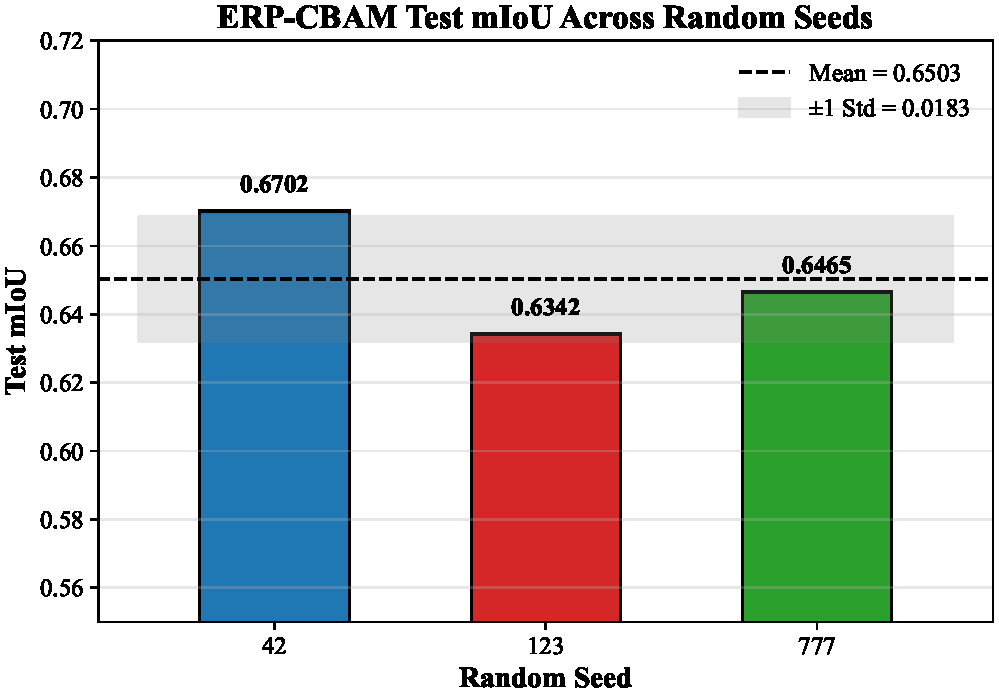
\includegraphics[width=0.85\textwidth]{figures/figS1_multiseed_test_miou_bar.pdf}
\caption{Test mIoU of ERP-CBAM for seeds $42$, $123$ and $777$.
The dashed line is the mean ($0.6503$); the band is $\pm 1$ standard
deviation ($0.0183$).}
\label{fig:seedbar}
\end{figure}

\begin{figure}[t]
\centering
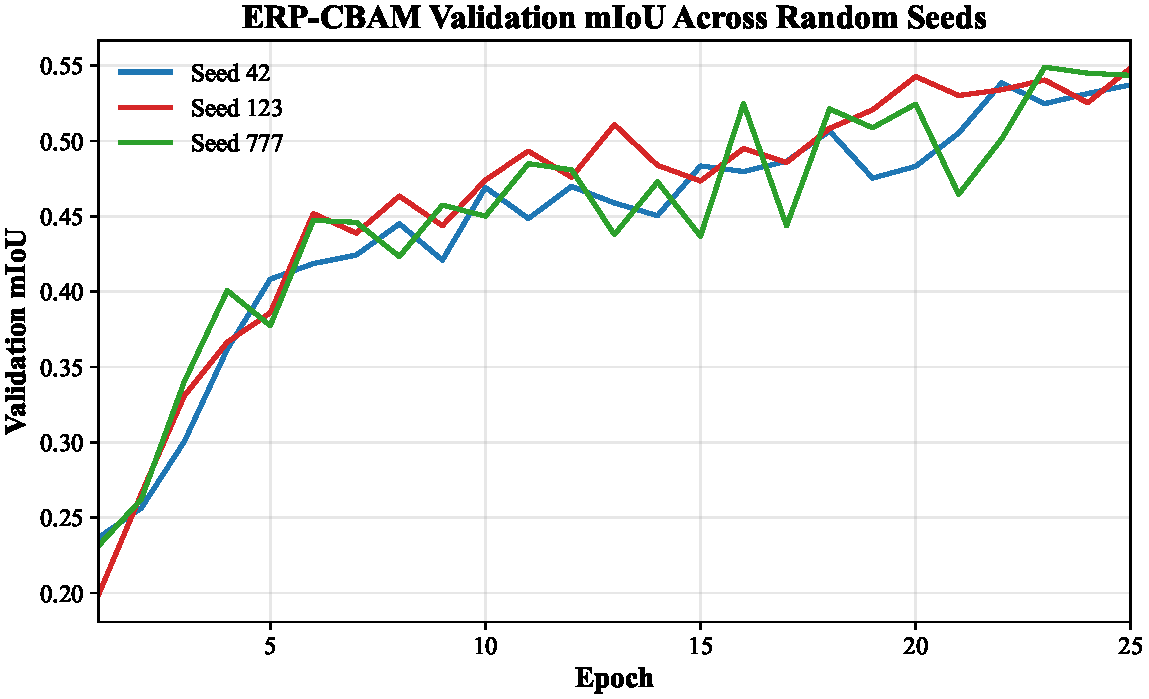
\includegraphics[width=0.85\textwidth]{figures/figS2_multiseed_val_miou.pdf}
\caption{Validation mIoU over 25 training epochs for the three seeded
ERP-CBAM runs. The trajectories remain closely aligned.}
\label{fig:seedval}
\end{figure}

\begin{figure}[t]
\centering
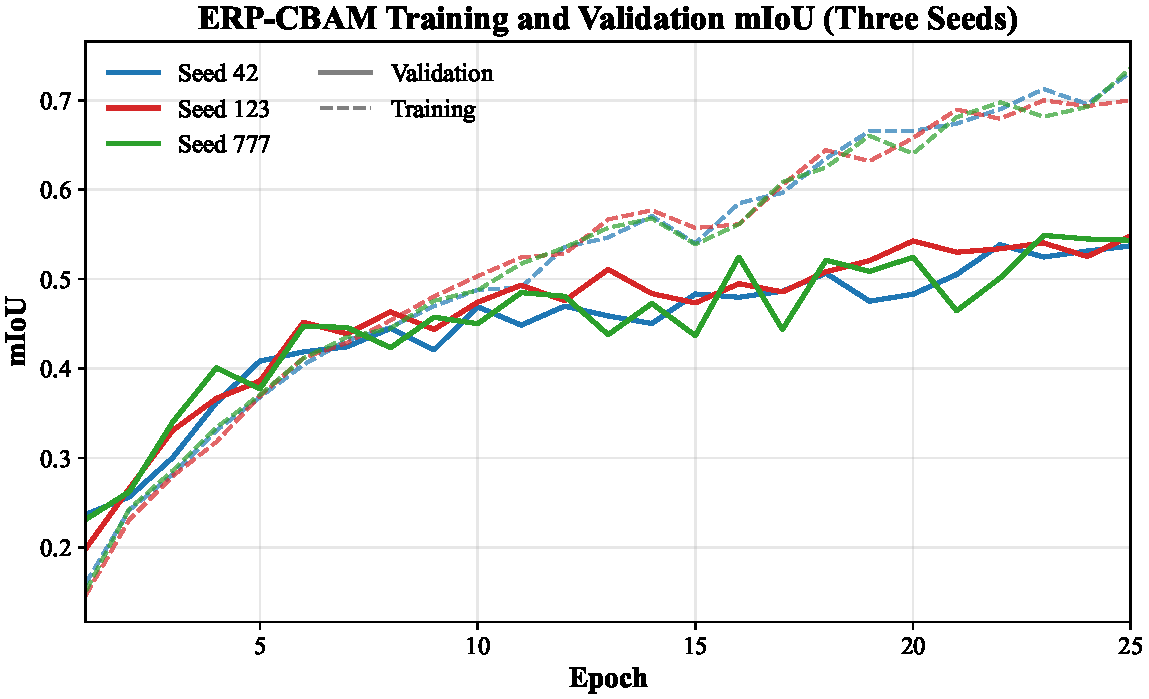
\includegraphics[width=0.85\textwidth]{figures/figS3_multiseed_train_val_miou.pdf}
\caption{Training and validation mIoU for the three seeds.
Solid lines: validation; dashed lines: training.}
\label{fig:seedtv}
\end{figure}

\begin{figure}[t]
\centering
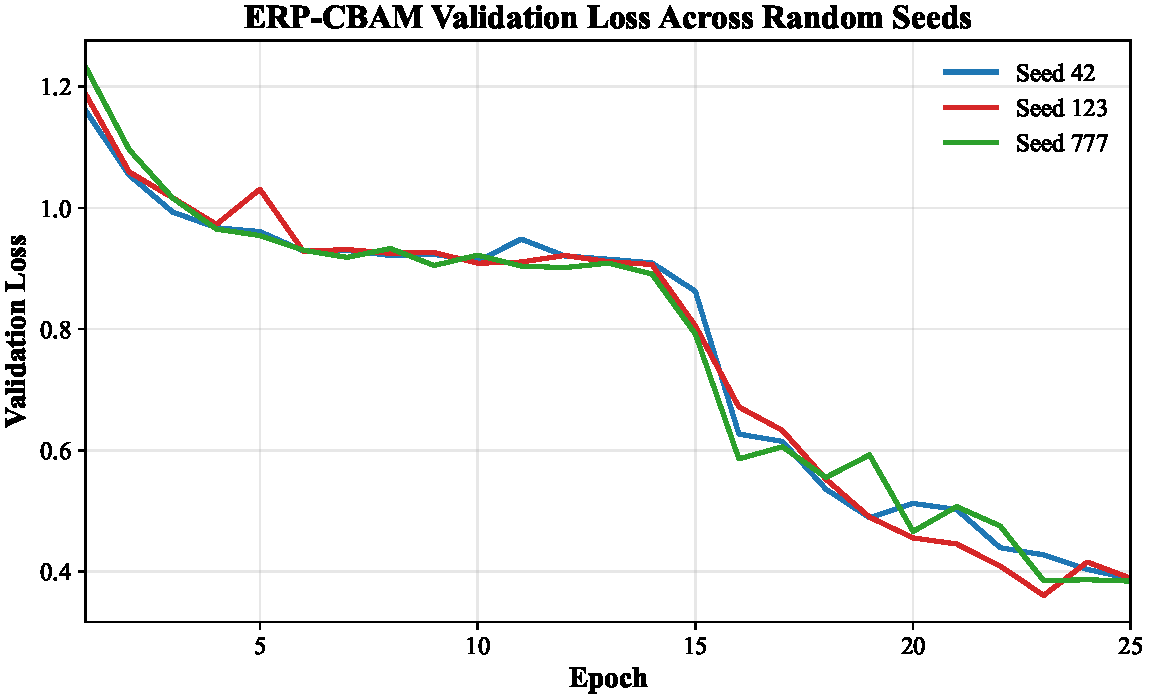
\includegraphics[width=0.85\textwidth]{figures/figS4_multiseed_val_loss.pdf}
\caption{Validation loss over 25 epochs for seeds $42$, $123$ and
$777$.}
\label{fig:seedloss}
\end{figure}

\section{Computational cost of ERP video inference}
\label{sec:compute}

ERP-CBAM is DeepLabv3+ with latitude-weighted spatial attention.
It cannot be substantially faster than its host.
Table~\ref{tab:compute} shows $+0.012$~M parameters ($+0.05\%$) and
$+0.017$~GFLOPs ($+0.007\%$) at $1440\times736$.
On the RTX~5070~Ti, ERP-CBAM measures $79.1$~FPS ($12.64$~ms) against
$86.8$~FPS for DeepLabv3+ ($11.53$~ms), about $9\%$ slower.
The claim that stands is that the mIoU gain is obtained inside the
DeepLabv3+ compute envelope, not that ERP-CBAM is the fastest model.

\begin{table}[t]
\centering
\caption{ERP video inference cost ($1440\times736$, batch~$=1$,
11~classes). Parameters and GFLOPs are hardware-independent.
Latency/FPS: single forward pass on RTX~5070~Ti.}
\label{tab:compute}
\scriptsize
\begin{tabular}{lccccc}
\toprule
\textbf{Model} & \textbf{Params (M)} & \textbf{GFLOPs} &
\textbf{Peak mem. (MB)} & \textbf{Latency (ms)} & \textbf{FPS} \\
\midrule
U-Net     & 24.44 & 255.8 & 623  & 16.57 & 60.3 \\
U-Net++   & 26.08 & 597.6 & 1536 & 38.46 & 26.0 \\
PSPNet    & 21.48 &  77.2 & 460  &  4.83 & 206.9 \\
DeepLabv3+& 22.44 & 255.3 & 774  & 11.53 & 86.8 \\
ERP-CBAM  & 22.45 & 255.4 & 861  & 12.64 & 79.1 \\
\bottomrule
\end{tabular}
\end{table}

\begin{figure}[t]
\centering
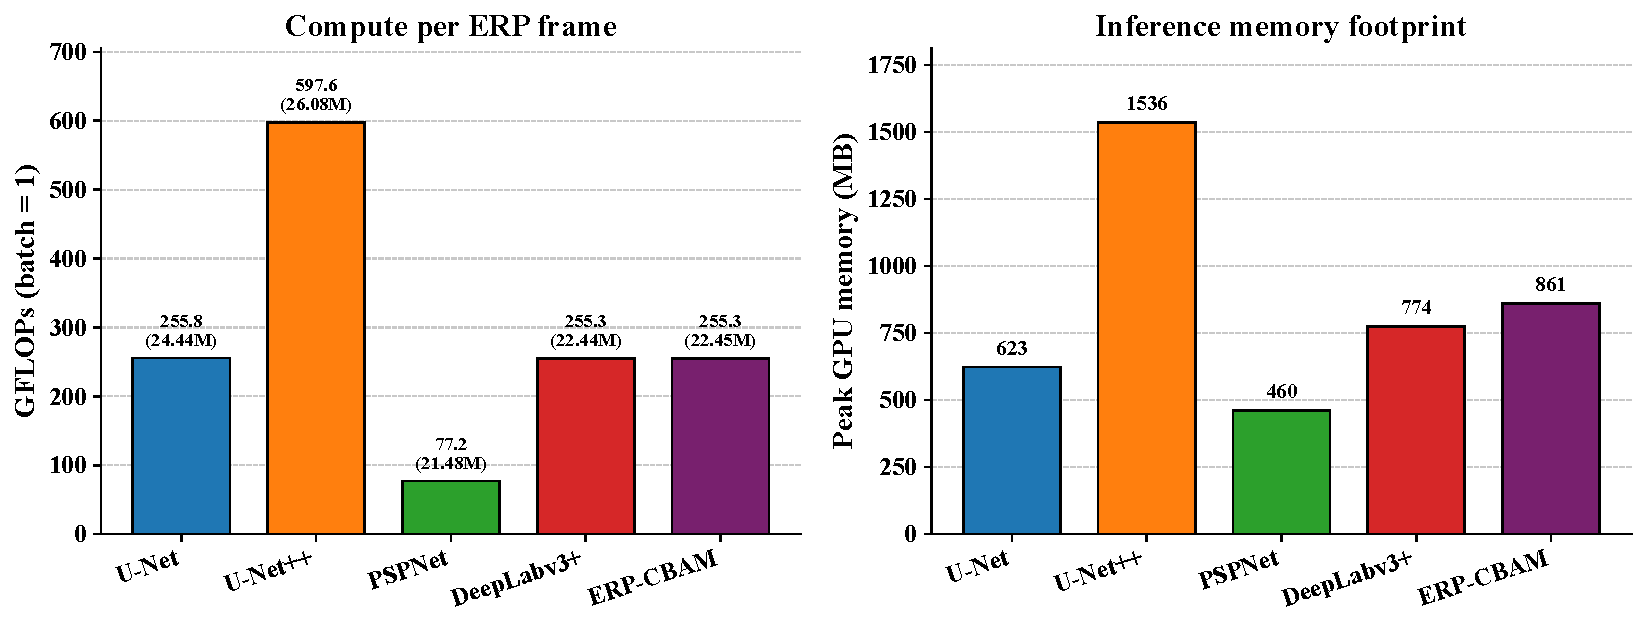
\includegraphics[width=0.98\textwidth]{figures/figS5_compute_efficiency.pdf}
\caption{Left: GFLOPs per ERP frame (parameter count in parentheses).
Right: peak GPU memory. ERP-CBAM is indistinguishable from DeepLabv3+
on FLOPs and stays below 1~GB of inference memory.}
\label{fig:compute}
\end{figure}

\section{Full metric comparison}
\label{sec:metrics}

Table~\ref{tab:main} repeats the nine-metric test-set comparison.
Mean IoU and Balanced Accuracy are the primary ranking metrics because
PanoDive360 is strongly imbalanced (diver in 1{,}010 of 1{,}052 frames;
dolphin in 27).
Figures~\ref{fig:radar} and~\ref{fig:bar} visualise the same numbers.

\begin{table}[t]
\centering
\caption{PanoDive360 test set. Best per column in bold.}
\label{tab:main}
\scriptsize
\setlength{\tabcolsep}{3.5pt}
\begin{tabular}{lccccccccc}
\toprule
Model & Acc. & mIoU & Prec. & Rec. & F1 & Dice & Spec. & Bal.Acc. & MCC \\
\midrule
U-Net      & 0.961 & 0.444 & 0.741 & 0.672 & 0.663 & 0.663 & 0.983 & 0.828 & 0.680 \\
U-Net++    & 0.959 & 0.437 & 0.768 & 0.647 & 0.646 & 0.646 & 0.981 & 0.814 & 0.674 \\
PSPNet     & 0.923 & 0.371 & 0.780 & 0.470 & 0.461 & 0.461 & 0.966 & 0.718 & 0.519 \\
DeepLabv3+ & 0.947 & 0.536 & 0.780 & 0.680 & 0.655 & 0.655 & 0.979 & 0.830 & 0.726 \\
ERP-CBAM   & 0.955 & \textbf{0.662} & 0.773 & \textbf{0.758} & \textbf{0.726}
           & \textbf{0.831} & \textbf{0.983} & \textbf{0.870} & 0.716 \\
\bottomrule
\end{tabular}
\end{table}

\begin{figure}[t]
\centering
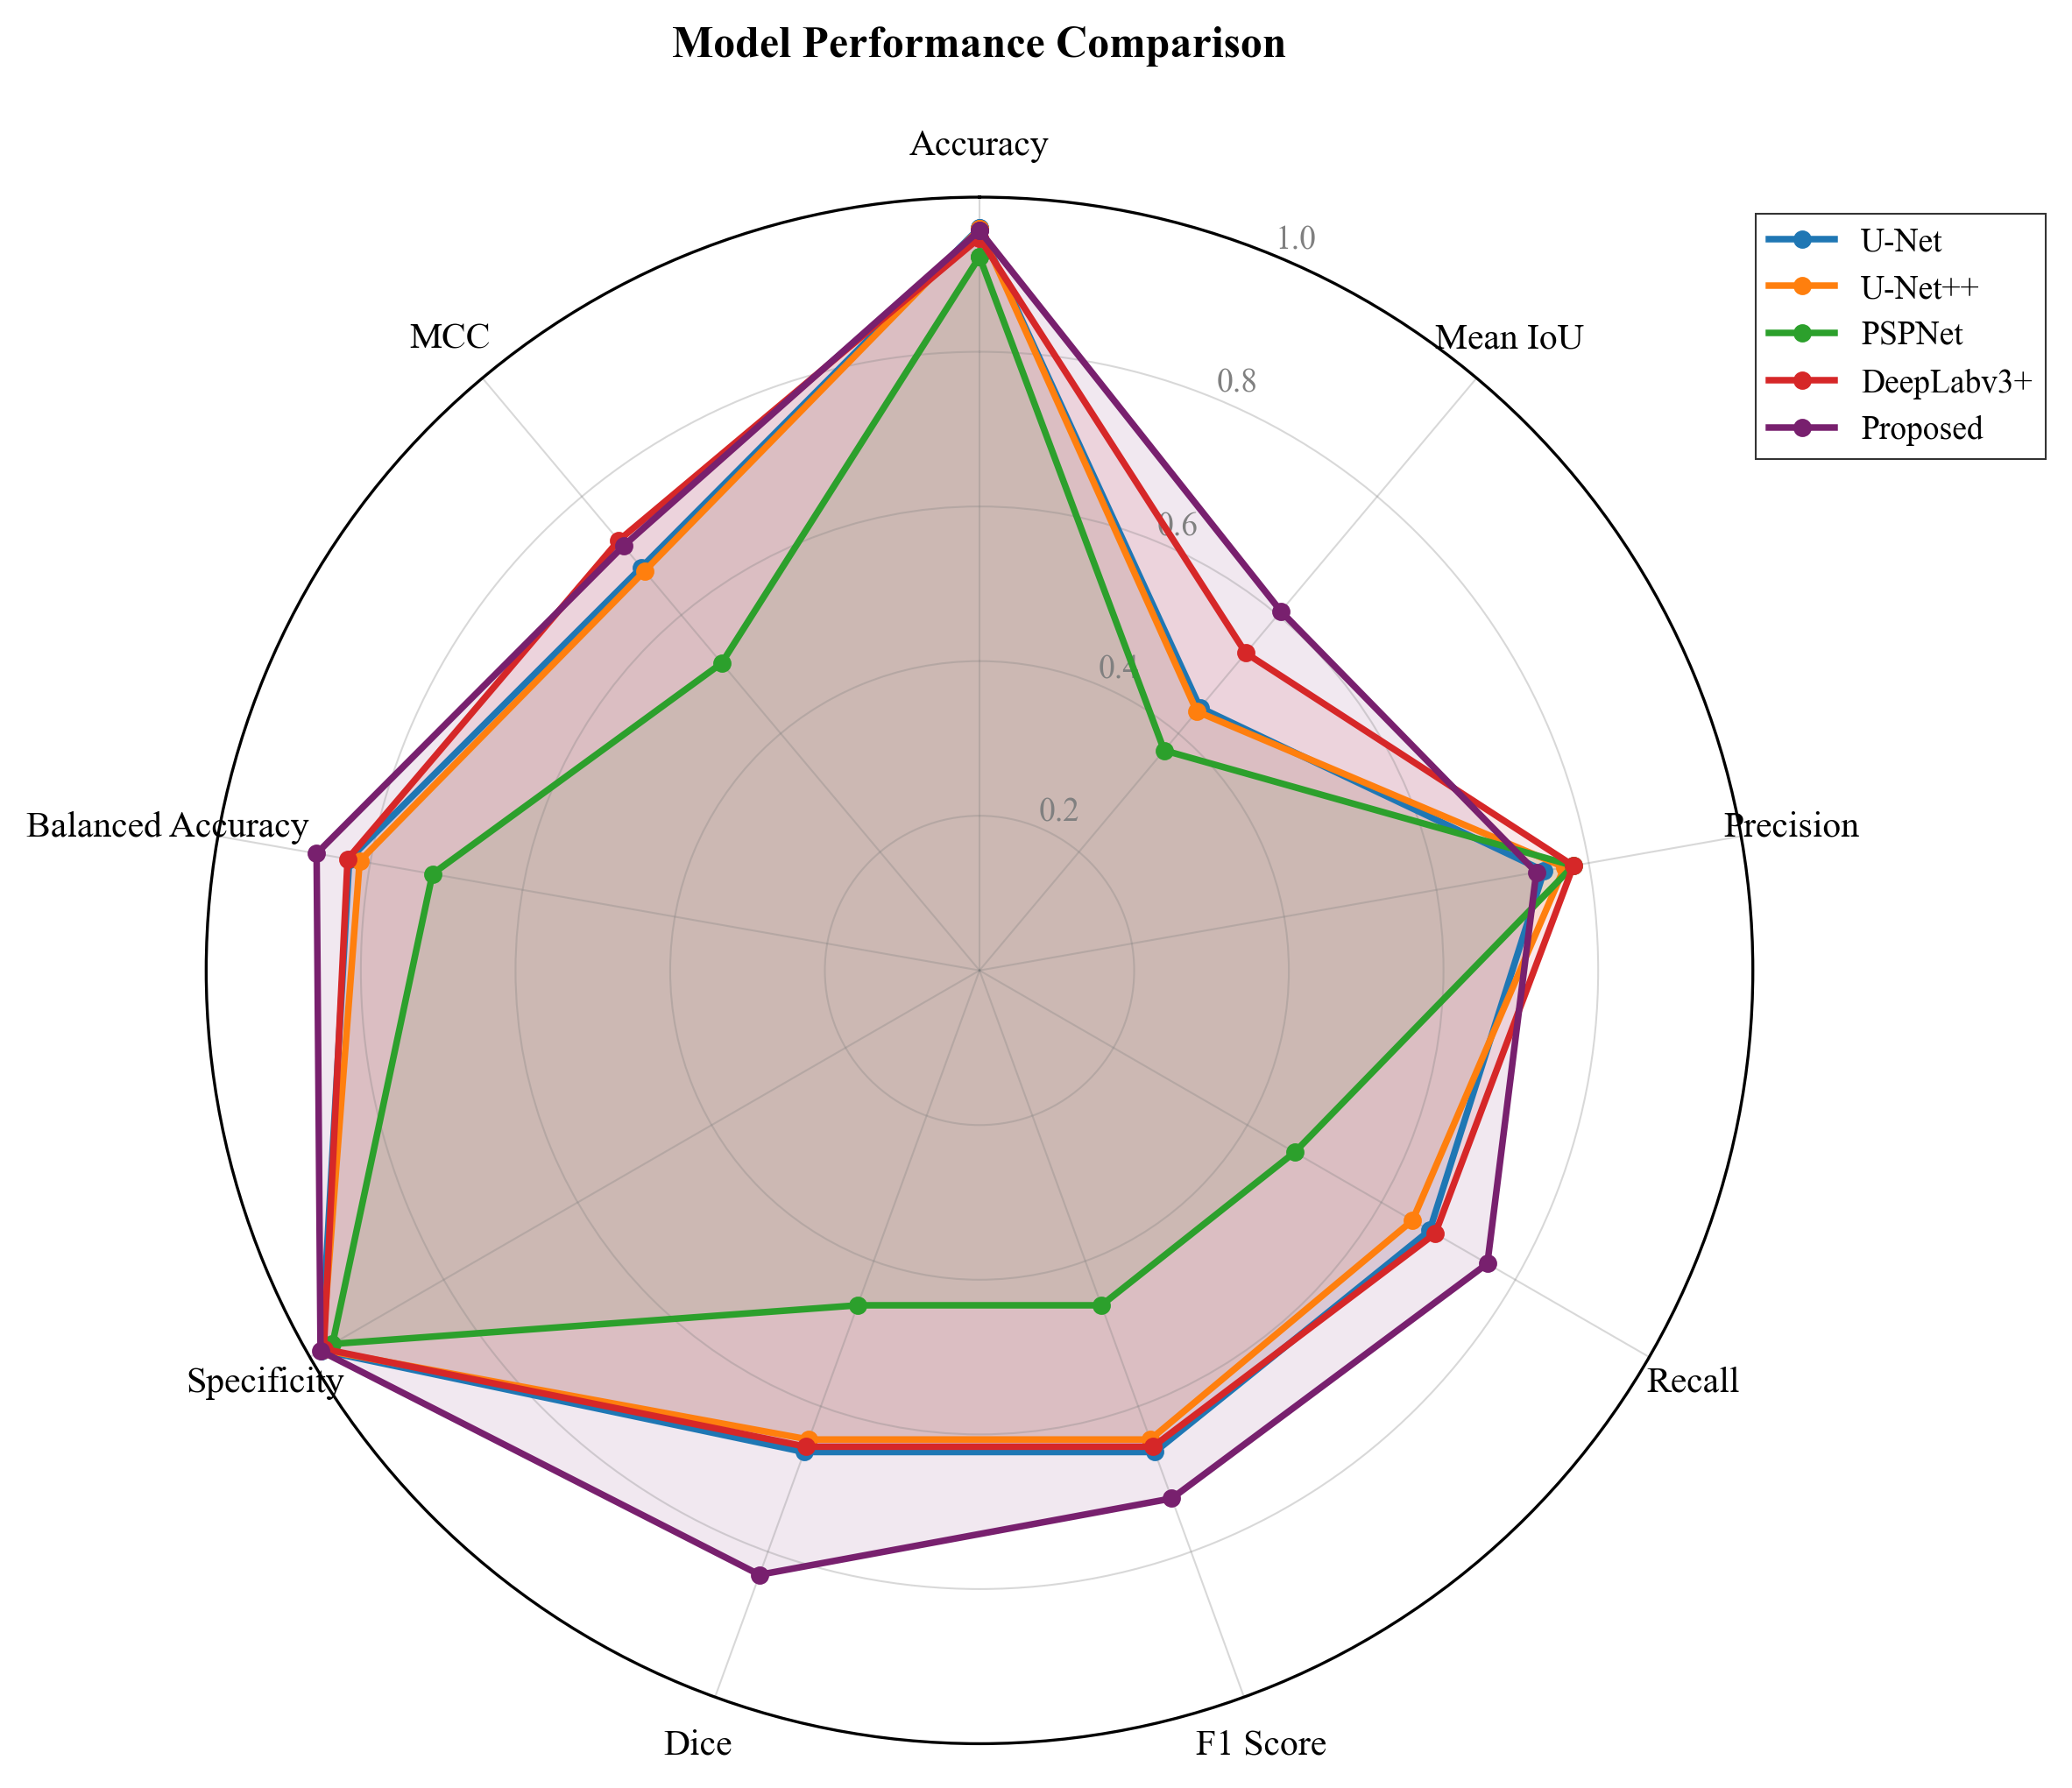
\includegraphics[width=0.72\textwidth]{figures/figS6_radar_metrics.png}
\caption{Radar comparison of the five CNNs across eight segmentation
metrics on the PanoDive360 test set.}
\label{fig:radar}
\end{figure}

\begin{figure}[t]
\centering
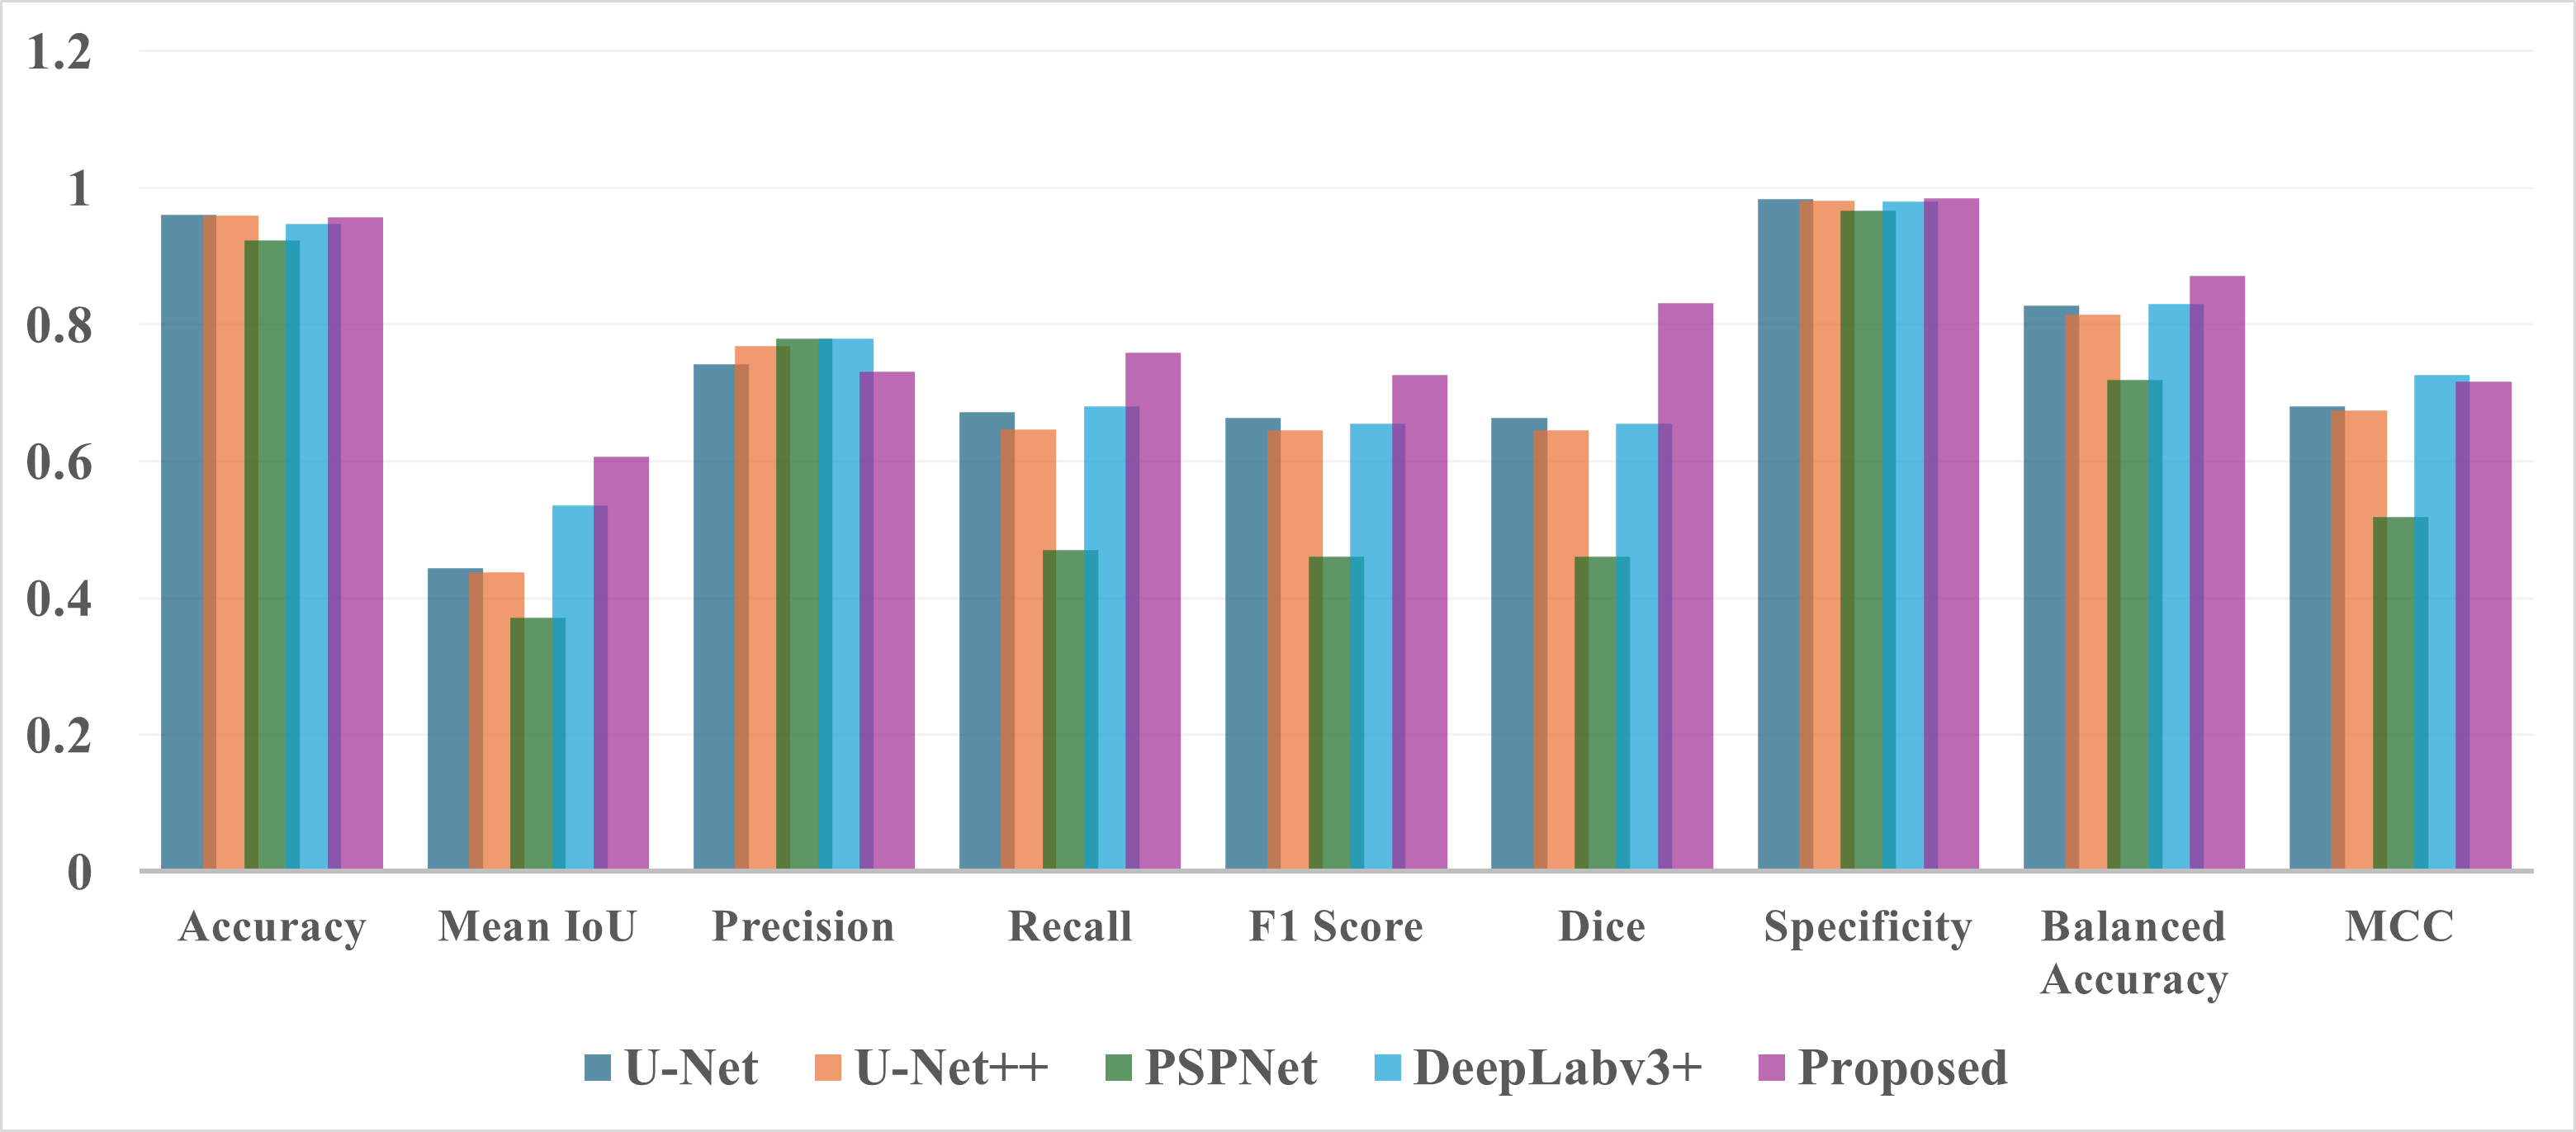
\includegraphics[width=0.92\textwidth]{figures/figS7_grouped_bar_metrics.png}
\caption{Grouped bar chart of the same nine metrics.}
\label{fig:bar}
\end{figure}

\section{Per-class IoU}
\label{sec:perclass}

\begin{table}[t]
\centering
\caption{Per-class IoU and precision for ERP-CBAM on the test set.
Instance counts are dataset-wide, not test-only.}
\label{tab:perclass}
\begin{tabular}{lccc}
\toprule
\textbf{Class} & \textbf{IoU} & \textbf{Precision} & \textbf{Instances} \\
\midrule
Background & 0.958 & 0.982 & 1{,}025 \\
Diver      & 0.741 & 0.856 & 1{,}010 \\
Shark      & 0.838 & 0.909 & 310 \\
Fish       & 0.499 & 0.625 & 267 \\
Sea Turtle & 0.845 & 0.875 & 41 \\
Dolphin    & 0.107 & 0.335 & 27 \\
Sea Lion   & 0.779 & 0.901 & 68 \\
Coral      & 0.561 & 0.787 & 96 \\
Shipwreck  & 0.790 & 0.879 & 275 \\
Seaweed    & 0.606 & 0.703 & 323 \\
Rock       & 0.564 & 0.662 & 272 \\
\bottomrule
\end{tabular}
\end{table}

Dolphin (IoU~$0.107$) is a data-limited outlier (27 instances), not an
architectural failure.
Sea turtle remains strong (IoU~$0.845$) despite only 41 instances.

\section{Ablation}
\label{sec:ablation}

\begin{table}[t]
\centering
\caption{ERP-CBAM ablation on the PanoDive360 test set.
CA~=~channel attention, SA~=~spatial attention, Lat.~=~latitude
weighting.}
\label{tab:ablation}
\scriptsize
\begin{tabular}{lccccccc}
\toprule
Variant & Acc. & mIoU & Rec. & F1 & Dice & Bal.Acc. & MCC \\
\midrule
DeepLabv3+              & 0.947 & 0.536 & 0.680 & 0.655 & 0.655 & 0.830 & 0.726 \\
Baseline + CBAM         & 0.920 & 0.409 & 0.544 & 0.543 & 0.824 & 0.752 & 0.525 \\
ERP-CBAM w/o ERP        & 0.956 & 0.635 & 0.705 & 0.751 & 0.907 & 0.839 & 0.737 \\
ERP-CBAM w/o Lat.       & 0.959 & 0.637 & 0.723 & 0.750 & 0.908 & 0.851 & 0.737 \\
ERP-CBAM w/o CA         & 0.951 & 0.569 & 0.652 & 0.690 & 0.896 & 0.815 & 0.690 \\
ERP-CBAM (full)         & 0.955 & \textbf{0.662} & \textbf{0.758} & \textbf{0.726}
                        & 0.831 & \textbf{0.870} & 0.716 \\
\bottomrule
\end{tabular}
\end{table}

Standard CBAM without latitude weighting \emph{decreases} mIoU from
$0.536$ to $0.409$.
Latitude weighting is the main driver of the balanced-metric gains
(recall $0.723\rightarrow0.758$, balanced accuracy
$0.851\rightarrow0.870$).

\section{Dataset class inventory}
\label{sec:data}

PanoDive360 contains 1{,}052 pixel-annotated monoscopic ERP stills from
30 publicly shared 4K 360-degree videos, 11 classes, 2:1 aspect.
Figure~\ref{fig:dist} shows the instance histogram.

\begin{figure}[t]
\centering
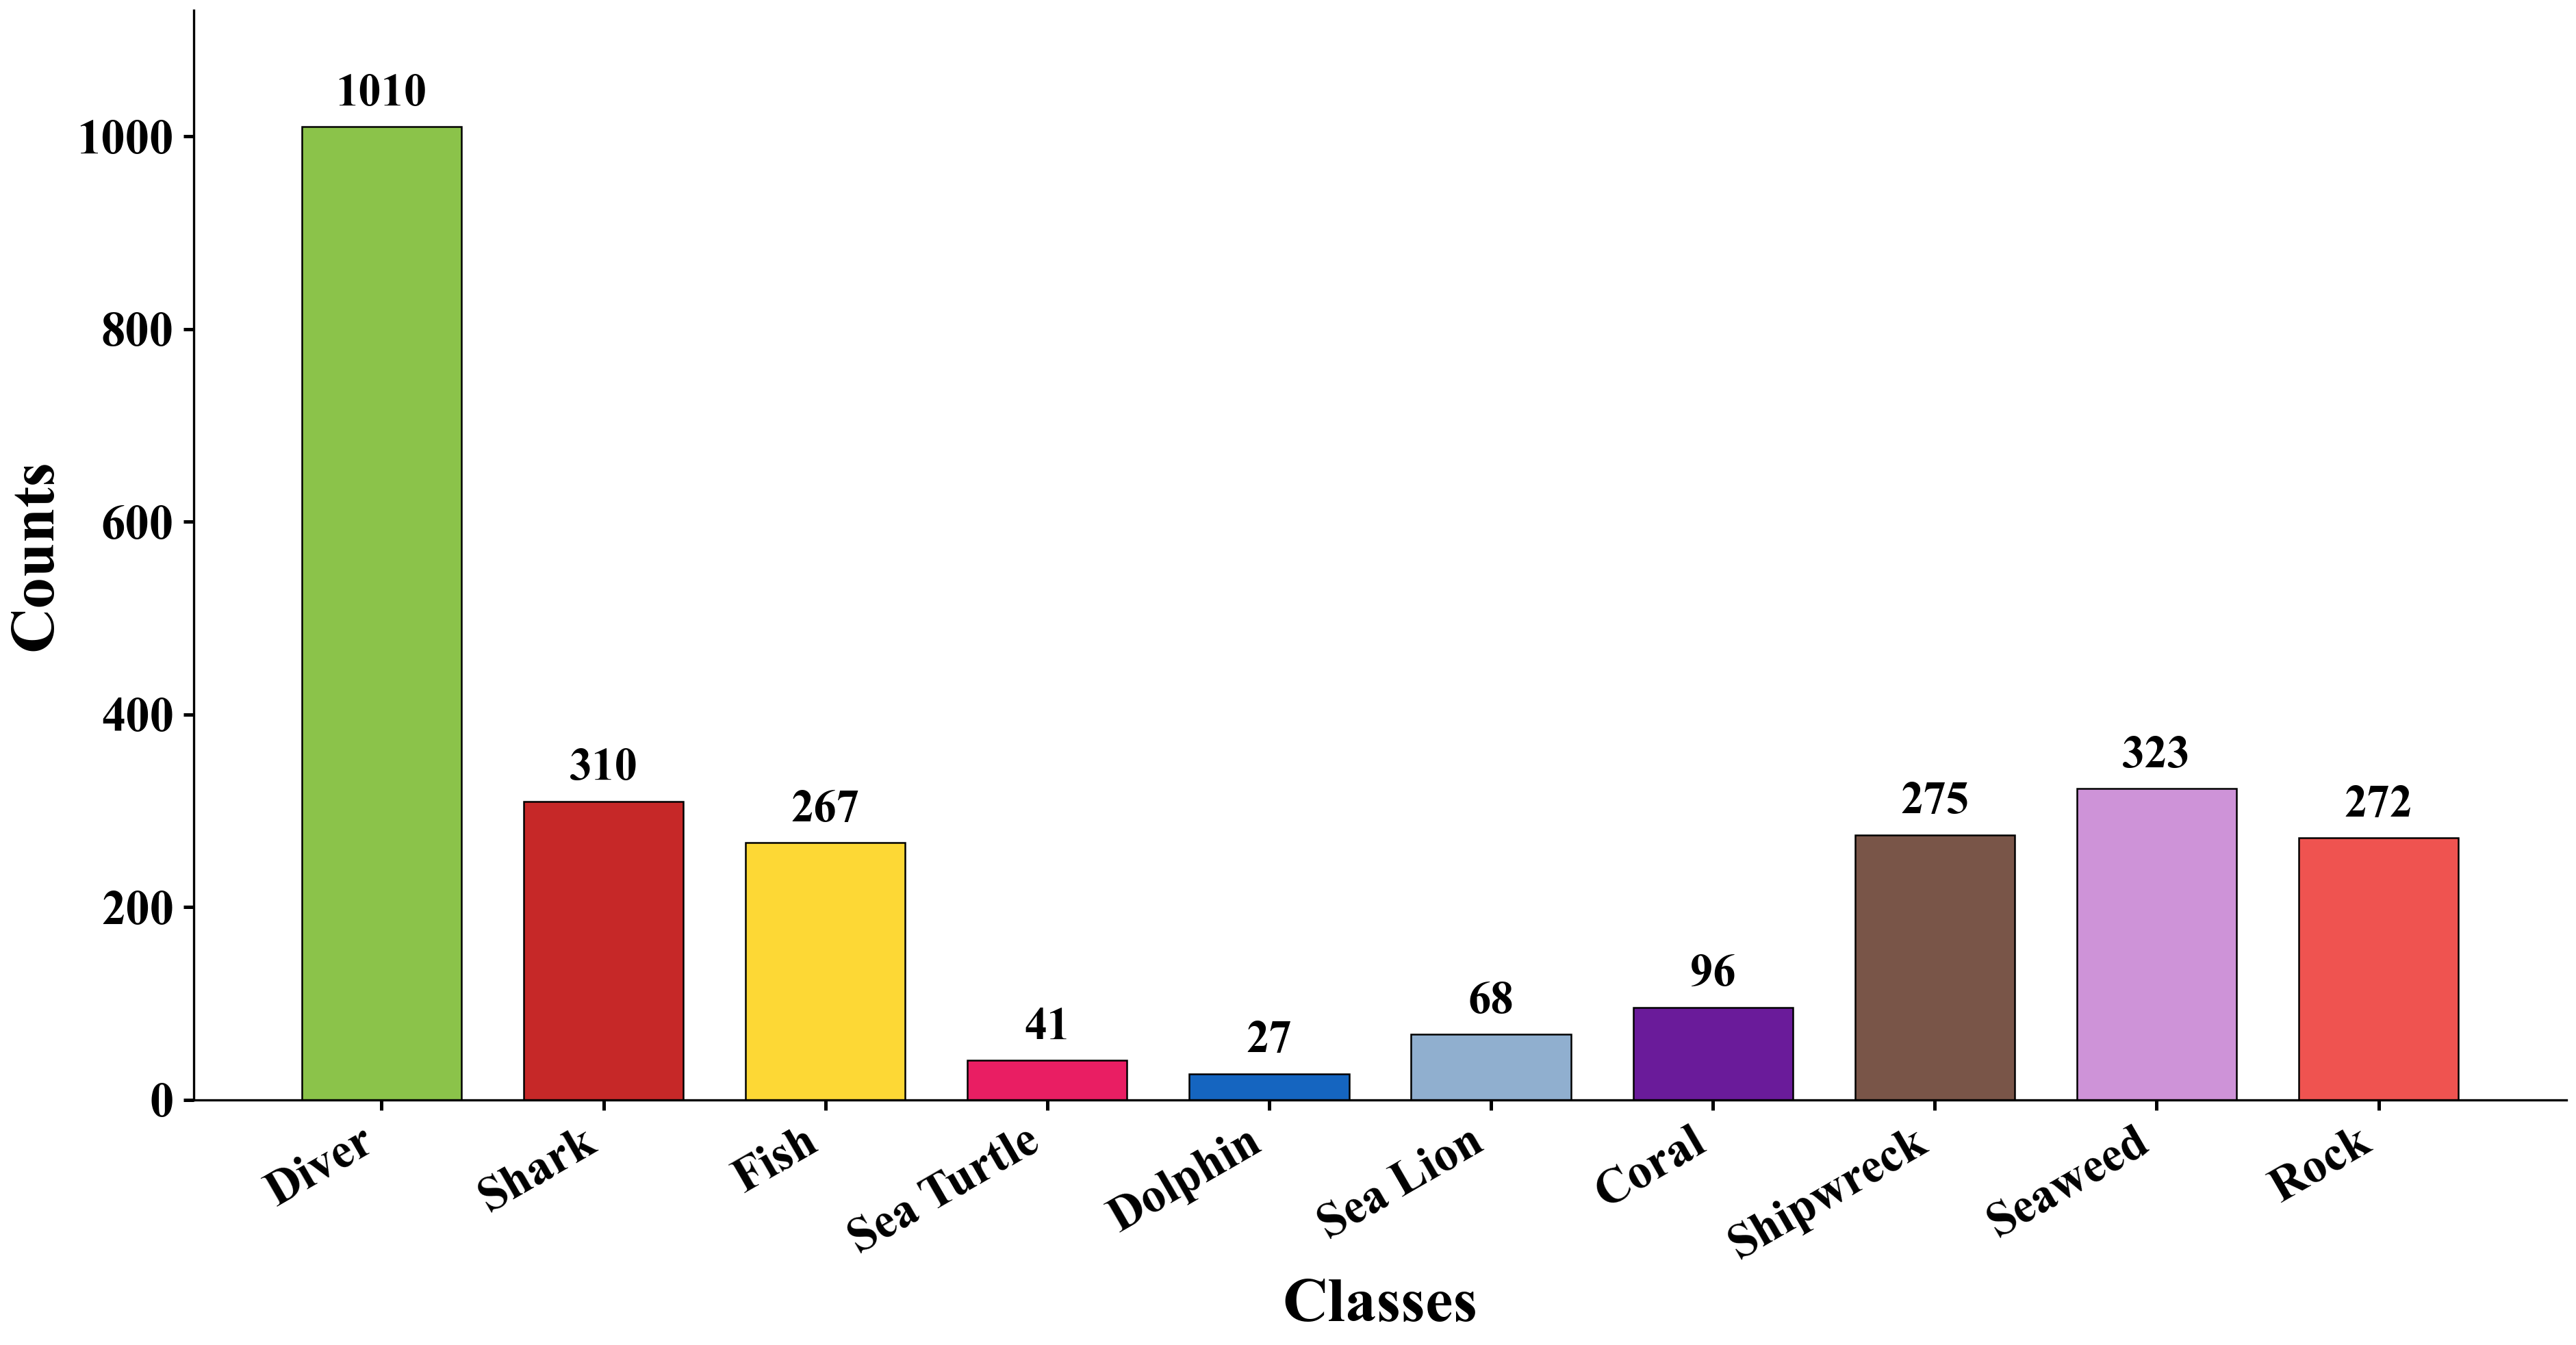
\includegraphics[width=0.78\textwidth]{figures/figS8_class_distribution.png}
\caption{Class instance counts. Diver dominates (1{,}010); dolphin (27)
and sea turtle (41) are rare.}
\label{fig:dist}
\end{figure}

\end{document}
